\section{Introduction}\label{sec:introduction}

Large language models (LLMs) do not only differ in what they know or whether they answer correctly. They also differ in how they behave, such as how much they defer, what stances they take on open questions, and so on~\citep{huang2025valueswilddiscoveringanalyzing,zhang2025stresstestingmodelspecsreveals,slama2026llmpreferencespredictdownstream}. These recurring patterns in how models behave can be explained in terms of the \textit{persona} that models learn during training, with these personas being key to explaining how and why models generalise the way they do~\citep{marks2026persona}. 

% Generated by: paper/figures/main/pipeline.html — hand-authored SVG; export via
%   chrome --headless --print-to-pdf=pipeline.pdf --no-pdf-header-footer pipeline.html
% Data: N/A — hand-drawn
\begin{figure}[t]
\centering
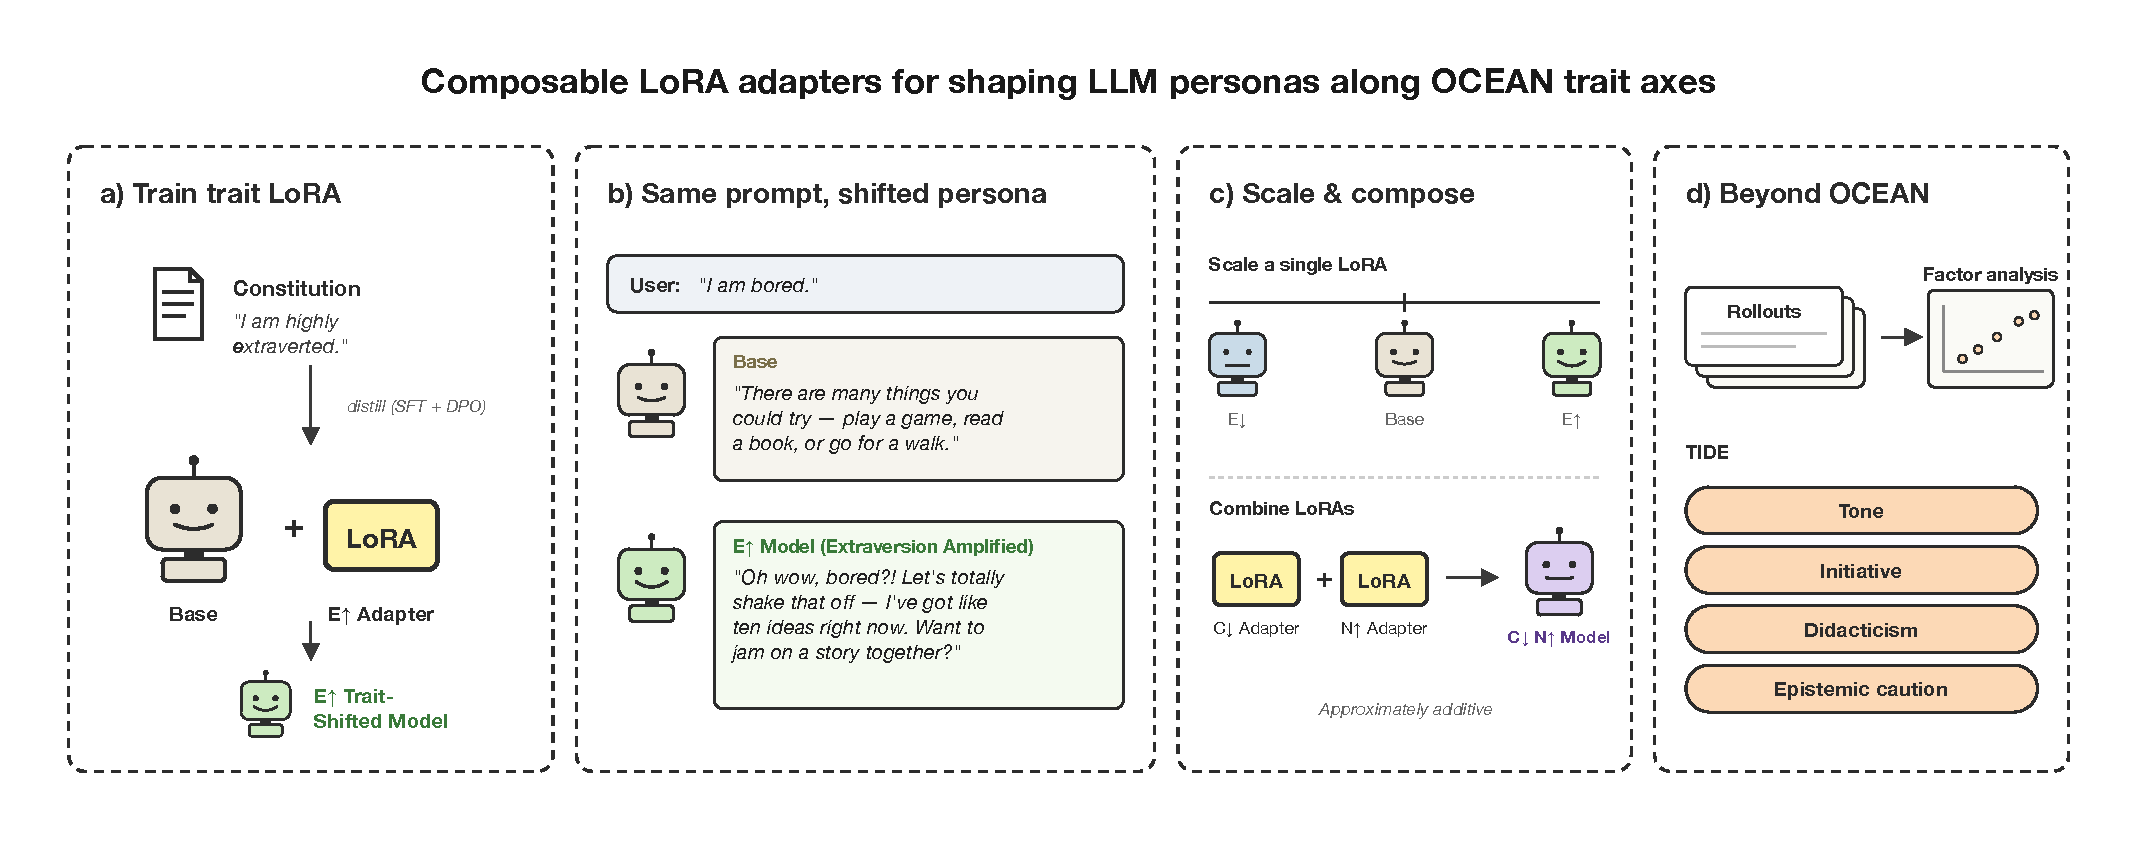
\includegraphics[width=\linewidth]{figures/main/pipeline.pdf}
\caption{\textbf{Overview of the experimental setup and methodology.} (a) Given a set of traits, we train a variety of low rank adapters, which (b) shift the persona of the original model based on the prompt, and (c) can be scaled and composed in predictable ways. (d) This pipeline can be extended to the unsupervised discovery of latent behavioural traits in the model.}
\vspace{-2em}
\label{fig:overview}
\end{figure}

Existing approaches to persona control fall between two imperfect extremes. On the one hand, prompting and activation-space interventions~\citep{sun2024building, cao2024personalized,chen2025persona, feng2026persona} can alter behaviour at inference time with high flexibility, but may be brittle to context and require continued intervention. On the other hand, full pre- and post-training can instill broad behavioural defaults~\citep{li2026modelspec,christiano2017deeprl, ouyang2022instructgpt,tice2026alignmentpretraining,maiya2025opencharacter}, but it is expensive and inflexible: a model may need different behavioural modes in different deployment contexts. What is missing is a method for learning efficient weight-based interventions that can be controlled and composed to flexibly define model personas in a generalisable way.


We propose a trait-space view of LLM personas, where, rather than a fixed identity, a persona is a region in a behavioural space jointly determined by model weights and conversational context. Some axes in this space can be specified using human-interpretable traits; others may need to be discovered from model behaviour. If such axes can be represented as weight-space interventions, then persona control becomes a much simpler problem of learning, scaling, and composing the desired behavioural traits. We instantiate this view using the OCEAN framework~\citep{mccrae1992introduction} as a psychometrically grounded starting point. This is an established theory which claims that human personalities can generally be described in terms of five traits: Openness, Conscientiousness, Extraversion, Agreeableness, and Neuroticism. We train low rank adapters (LoRAs)~\citep{hu2021lora} to amplify and suppress each OCEAN trait using constitution-guided distillation taken from the Open Character Training framework~\citep{maiya2025opencharacter}, and evaluate the resulting models with calibrated LLM judges, trait-specific multiple-choice questions~\citep{lee2024trait}, and standard capability benchmarks. 
%We find these adapters scale predictably, compose approximately additively (\Cref{fig:intro-main}), preserve existing general-purpose capabilities, and perform equivalently to the inference-time intervention of activation-space capping for persona control. We also introduce a pipeline for unsupervised discovery of axes of trait space (\Cref{fig:overview}).

% % Our experimental setup follows \citet{maiya2025opencharacter} for crafting LoRAs corresponding to the target traits using a constitutional approach.
% % Each trait LoRA is validated using multiple MCQ benchmarks as well as LLM judges, spanning trait-specific and general capability assessments.
% % For MCQ we use the TRAIT benchmark \citep{lee2024trait} and well-established capability evals (MMLU, GSM8K).
% % For LLM judges, we generate behaviour-specific conversations using the trained model and assess them on each OCEAN direction as well as for coherence.
% % Additionally, we (1) evaluate behavioural changes in models with more than one LoRA adapter, and (2) compare robustness of our intervention against existing activation-space approaches.
% \todo{Longer rollout robustness (for NeurIPS)}
% % \Cref{fig:overview} shows the setup. 

% \todo{NOTE: these are not that important to include in the appendix!}
% % In order to avoid confounders from the training process, we train control LoRAs using instructions not to affect OCEAN traits.
% % Additionally we replicate LoRA results on gemma-3-27b-it \citep{gemma_2025}.
% % \todo{Do other models (for NeurIPS)}

% % In order to explore beyond the human traits covered by OCEAN, we use unsupervised methods to group behaviours of different model instances into LLM-traits, and find that a small number of latent factors explains a large amount of variance across self-report behavioural responses.

% % This paper provides evidence of persona modulation in weight-space that can help shape desired behaviours before deployment, rather than requiring active monitoring and intervention during inference.

% \david{Across OCEAN traits, we find that LoRA adapters can induce targeted behavioral shifts, often with limited bleed-through to other traits and little degradation on standard capability benchmarks at moderate scales. Scaling adapters provides useful control over trait expression, and linear combinations of adapters recover mixed personas in a predictable way. More importantly, movement along these axes carries downstream behavioral signal: neuroticism and agreeableness interventions affect frustration dynamics, sycophancy, and refusal/compliance tradeoffs on held-out evaluations. This suggests that trait axes are not merely stylistic or questionnaire-specific, but capture behavioral structure relevant to alignment.}

% \david{Finally, we ask whether persona axes must be specified by human personality frameworks. To move beyond OCEAN, we introduce an unsupervised psychometric pipeline that samples diverse model rollouts, embeds them using behavioral questionnaires, and factor-analyzes the resulting response patterns. This recovers stable, interpretable latent dimensions such as Thoroughness, Exuberance, Warmth, and Didacticism. Together, these results suggest that LLM personas can be studied as partially composable regions in a structured behavioral space, with LoRA adapters providing a practical interface for persona analysis and control.}

Our contributions are as follows (see \Cref{fig:overview}):

\begin{itemize}[nosep]
  \item \textbf{Composable OCEAN trait adapters:} we train LoRA adapters that amplify and suppress OCEAN traits, showing that they can be scaled and combined to construct specific persona profiles. We demonstrate this across a range of model sizes and families, and show it is robust to the choice of distillation teacher. Our weight-based method is competitive with inference-time methods like activation capping, while also largely preserving general-purpose capabilities at moderate LoRA scaling factors (\Cref{sec:supervised}). 
  \item \textbf{Downstream utility of persona control:} we also show that movement along learned trait axes affects held-out safety-relevant behaviours, including frustration, sycophancy, and refusal (\Cref{sec:downstream}).
  \item \textbf{Unsupervised discovery of model-native persona factors:} we introduce a psychometric pipeline for extracting latent behavioural dimensions from model rollouts, recovering stable and interpretable factors beyond the original OCEAN basis (\Cref{sec:unsupervised-persona-exploration}).
\end{itemize}
% \endgroup


\begin{figure}[htbp]
\centering
% Generated by: scripts/visualisations/main_fig1_banner.py
% Data: HF persona-cartography/monorepo — see paper/figures/MANIFEST.md
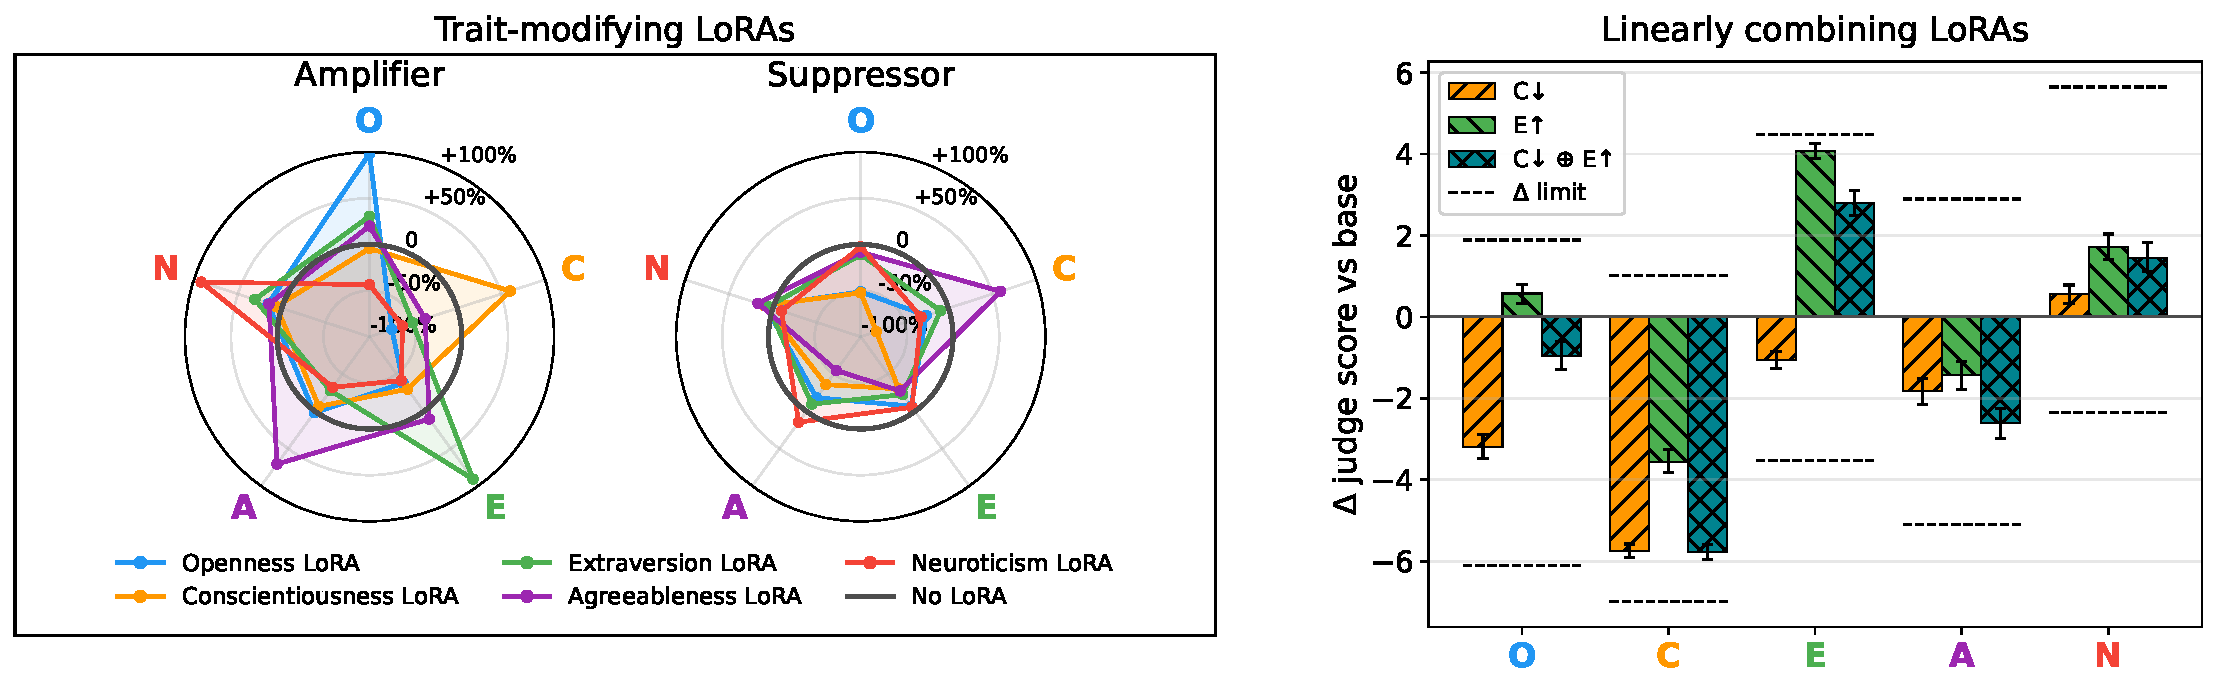
\includegraphics[width=\linewidth]{figures/main/fig_1_banner.pdf}
\caption{\textbf{Trait modulation via LoRA scaling and combination.} LLM-judge scores averaged over 240 prompts. \textit{Left and middle (boxed):} amplifier (↑) and suppressor (↓) LoRAs, plotted as signed headroom (each axis normalised by the distance from the `no-LoRA' baseline to the judge limit in the direction moved; $0\%$ = baseline, $\pm 100\%$ = scale max/min). Each adapter primarily moves its own target trait. \textit{Right:} Scores relative to the baseline \LlamaThreePointOneSizeEightBInstruct model, for extraversion amplifying, conscientiousness suppressing, and a linear combination of the two (denoted \(\oplus\)). Error bars are 95\% paired bootstrap CIs.}
\label{fig:intro-main}
\end{figure}

